%%%%(c)
%%%%(c)  This file is a portion of the source for the textbook
%%%%(c)
%%%%(c)    Abstract Algebra: Theory and Applications
%%%%(c)    Copyright 1997 by Thomas W. Judson
%%%%(c)
%%%%(c)  See the file COPYING.txt for copying conditions
%%%%(c)
%%%%(c)
\chap{Application: Further Topics in Cryptography}{further_crypt}

In this chapter we examine two specific topics in cryptography which are highly practical and are relatively recent developments: Diffie-Hellman key exchange (originated by Whitfield Diffie and Martin Hellman in 1976) and elliptic curve cryptography (proposed by Neal Koblitz and Victor Miller in 1985).
\medskip

\noindent
\emph{Prerequisites}: 
To understand this chapter, the reader should be familiar with the material in  Chapters~\ref{modular},\ref{functions}, and~\ref{groups}. We also make use of one important result from Chapter~\ref{poly}, but we only apply the result and don't make use of the proof itself.  
\bigskip

This chapter is written by Moses Marmolejo, with revisions by C.T.

\section{Diffie-Hellman key exchange}\label{sec:DHKE:1}

In order to share a private message over a public domain a sender must  "lock" or encrypt their message using a \emph{key}\index{key! in cryptogaphy}.  Recall from Section \ref{sec:crypt:overview}, that in cryptography a  key is a special piece of information (usually a number)  that is required to encrypt and decrypt data which is shared between the sender and receiver. There are generally three types of keys used: public, private and symmetric keys. A \emph{public key}\index{Public Key! in cryptography} can be widely distributed, and is typically used for encrypting messages.  For a public key to be effective, there must be a matching \emph{private key}\index{Private Key! in cryptography} which is known only to the receiver. The privat key can be used to decrypt the messages created using the public key.  Finally, a \emph{symmetric key}\index{Symmetric Key! in cryptography} is known by the sender and receiver, and is used to both encypt and decrypt messages.  Not all cryptosystems require all three kinds of keys, but every cryptosystem must have either a private key or a symmetric key.

  If a symmetric key is used, then both parties must share their key before they can begin communicating securely. The requirement of establishing a key exchange is so essential that it is embedded into almost every technology we use today.  Some examples of key exchange can be seen in media applications, cell phones, banking, online purchasing, and emails.  

 But what if the only way the two parties have to communicate is via a public network (such as the Internet), where eavesdroppers can listen in?  Under these conditions how can they possibly establish a shared key in such a way that no one else can find out?  The Diffie Hellman Key Exchange (DHKE) is one possible solution to the problem of creating a secret key over an insecure communication channel.  Note that the DHKE is not used for encryption/decryption of messages, but only to establish a key that can be used to encrypt/decrypt subsequent messages.  Follow the steps below to see the DHKE process.  

 \begin{enumerate}[Step 1.]
 \item First, Moses and Rachael agree upon a pair of numbers $p$ and $g$. $p$ is called the \term{modulus},while $g$ is called the \term{base}. These numbers are not secret, but Moses and Rachael do not care if eavesdroppers find out what $p$ and $g$ are. In practice, $p$ and $g$ are required to have certain properties (as explained below) to maximize secrecy.  However, the DHKE procedure still works for any values of $p$ and $g$.
\item Moses chooses a secret integer $n$, known only to himself.  He then computes $q$ where $q =\bmod(g^n,p)$, and sends Rachael the value of $q$. Rachael does not need to know the value of $n$.
\item Rachael similiarly chooses her own secret integer $m$, computes $r$ where $r =\bmod(g^m,p)$ and sends Moses the value of $r$.
\item Moses computes $ \bmod (r^n , p ) = k_M$;
\item Rachael computes $ \bmod (q^m , p ) = k_R$;
\end{enumerate} 
It turns out that when $k_R$ and $k_M$ are computed by the above procedure, then $k_R$ is always equal to $k_M$.  You will show this in the next exercise.  
\begin{figure}[htb]
	   \center{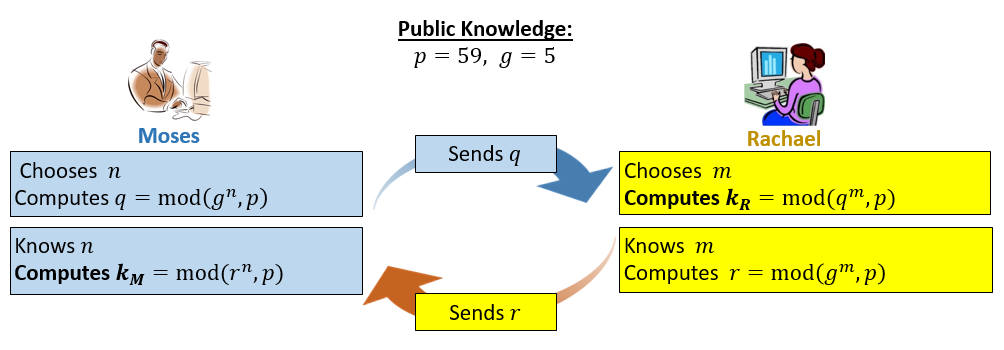
\includegraphics[width=4.5in]
	         {images/DHKE_1.png}}
	  \caption{\label{fig:DH:DHKE_1} Key exchange between Moses and Rachael using DHKE}
\end{figure}

\begin{exercise}{k1isk2}\\
Fill in the blanks in the following proof that  $k_R$ is always equal to  $k_M$.\\
  	\begin{proof} 
		\begin{align*} 
		k_R &=   \bmod (q^m , \underline{~~~~~~}) && \text{(definition of $k_M$)}
		\\&\equiv \bmod ((g^{\underline{~~~~~~}})^m , p) &&  \text{(substitution)}	
		\\&\equiv \bmod ((g^{\underline{~~~~~~}})^n , p) &&  \text{(rules of exponents)}
		\\&\equiv \bmod ((r^{\underline{~~~~~~}}) , p) &&  \text{(substitution)}		
		\\&= k_M
		\end{align*} 
   	If two numbers in $\mathbb{Z}_p$ are modular equivalent, then they are the same number. Thus, $k_R = k_M$ is a symmetric key, which we may refer to as $k$.\\

  	\end{proof}
\end{exercise}

Now that you understand the process for DHKE, follow the example below.  (Note that this example is just to give you the idea--it's much too simple to use in practical applications.)

 \begin{eg} Key Exchange between a sender and receiver (Moses and Rachael) using the DHKE is shown in the following steps.
\begin{enumerate}[Step 1.]
\item Prior to sending data, Moses and Rachael agree $p$ = 13 and $g$= 7; 
\item Moses chooses $n$ = 2, and sends Rachael $\bmod (7^2 , 13) = 10$;
\item Rachael chooses $m$ = 8, and sends Moses $\bmod (7^8  , 13) = 3 $;
\item Moses computes $\bmod ((3)^2 , 13 ) = 9$;
\item Rachael computes $\bmod ((10)^8 , 13 ) = 9$;
\item Moses and Rachael share the number 9;
\end{enumerate}
\end{eg}

%  \emph{Fermat's Little Theorem}\index{Fermat's Little Theorem! in cryptography} states that if $p$ is a prime number such that $p \nmid a$, and $a$ is an integer, then $1 \equiv \bmod(a^{p-1}, p)$.

%\begin{eg} Let $p = 5$ and $a = 1, 2, 3, 4 \text{ and } 5$
%$$ 5 \nmid 1 \implies \bmod(1^{5-1}, 5) \equiv 1$$
%$$ \bmod(1^{4}, 5) \equiv 1$$
%$$ \bmod(1, 5) \equiv 1$$
%$$ 5 \nmid 2 \implies \bmod(2^{5-1}, 5) \equiv 1$$
%$$ \bmod(2^{4}, 5) \equiv 1$$
%$$ \bmod(16, 5) \equiv 1$$
%$$ 5 \nmid 3 \implies \bmod(3^{5-1}, 5) \equiv 1$$
%$$ \bmod(3^{4}, 5) \equiv 1$$
%$$ \bmod(18	, 5) \equiv 1$$
%$$ 5 \nmid 4 \implies \bmod(4^{5-1}, 5) \equiv 1$$
%$$ \bmod(4^{4}, 5) \equiv 1$$
%$$ \bmod(256, 5) \equiv 1$$
%$$ 5 | 5 \text { (so the theorem does not apply)}$$
%$$ \bmod(5^{5-1}, 5) \equiv 0$$

%Since all values of $a$ such that $1 \leq a \leq p$ are congruent to $1$, then Fermat's Little Theorem tells us that $p$ is prime, but are there numbers that exist that pass Fermat's Little Theorem but are not prime?  The answer is yes, these numbers are called \emph{Lucas-Carmichael Numbers}\index{Lucas-Carmichael Numbers! in cryptogaphy}.  (or \emph{pseudoprimes}\index{Pseudoprimes}) 

Following the example above you can see that the DHKE requires that you raise a given number $g$ to a natural number (either $m$ or $n$) and take the result mod $p$. This operation is called \term{discrete exponentiation}. Calculating discrete exponentials with small values of $m$ or $n$ is manageable, but in practice the exponent $m$ or $n$ can be enormous, with hundreds of digits. It would seem that in this case discrete exponentiation would take a long, long time to compute.  But we can use the repeated squaring formula described in Section \ref{exercise:crypt:power} to speed up the process.  Create a spreadsheet using the repeated squaring formula to compute the following exercises.
 
\begin{exer}
Suppose you want to conduct a DHKE with one person, and you are given $p$ = 32452867; $g$ = 54321; and $n$ = 876.  
\begin{enumerate}[(a)]
\item What number do you send?  
%ans: mod((54321)876, 32,452,867) = 19,439,625

\item You are then sent 31975948, what is the shared key? 
%ans: K = mod((31,975,948)876, 32,452,867) = 16,045,878

\item If $m$ = 123 what number does the other party calculate for the shared key?
%ans: K = mod((19,439,625)123, 32,452,867) = 16,045,878
\end{enumerate}
\end{exer}

\begin{exer}
Suppose you want to conduct a DHKE with one person, and you are given $p$ = 86028157; $g$ = 98765; and $n$ = 123.  
\begin{enumerate}[(a)]
\item	What number do you send?  
%ans: mod((98765)123, 86,028,157) = 7,262,961

\item You are then sent 53161396, what is the shared key? 
%ans: K = mod((53,161,396)123, 86,028,157) = 35,164,864

\item If $m$ = 87 what number does the other party calculate for the shared key?
%ans: K = mod((7,262,961)87, 86,028,157) = 35,164,864
\end{enumerate}
\end{exer}
Now that we understand the DHKE process, let us try to understand why it effectively guarantees the secrecy of the shared key. First, we need to understand a little more about the operation of discrete exponentiation, which (as we have seen) is the foundation of the DHKE process. So we are going on a short digression, but don't worry--we will get back to the main point shortly. 

In previous math courses you learned that the inverse operation of exponentiation is taking the logarithm: for example, $2^3 = 8$ while $\log_{2}8 = 3$.  It is possible to do the same with discrete exponentiation: an inverse operation to discrete exponentiation is  referred to as `finding a \term{discrete logarithm} or (DL)'. Note that since discrete exponentiation involves raising to a power which is a natural number, a  DL will always be a natural number.   For example, since $\bmod(2^5,7)=4$, we could say that under multiplication mod 7,  $5$ is a DL  of $4$ with base $2$.

 Now why have we been saying, ``\emph{a} DL'' rather than ``\emph{the} DL''? Because  there happens to be more than one:

\begin{exercise}{DLex1}
\begin{enumerate}[(a)]
\item
Find all natural numbers $n$ such that $\bmod(2^n,7)=4$.  Use your result to complete the following sentence: ``Under multiplication mod 7, the discrete logarithm(s) of $4$ with base 2  are \ldots.''
%ans: n=2^(2+3x)
\item
Find all natural numbers $n$ such that $\bmod(2^n,7)=3$.  Use your result to complete the following sentence:  ``Under multiplication mod 7, the discrete logarithm(s) of $3$ with base 2 are \ldots.''
%ans: do not exist 
\item
Find all nonzero elements of $\mathbb{Z}_7 \setminus \{0\}$ which have no discrete logarithms with base 2.
%ans: 3,5,6
\item
Find all nonzero elements of $\mathbb{Z}_7 \setminus \{0\}$ which have no discrete logarithms with base 3.
%ans: all integers 1-6 are represented
\end{enumerate}
\end{exercise}

The preceding exercise points out some key issues with discrete logarithms. Sometimes there are lots of them, and sometimes there aren't any! These phenomena are related to the one-to-oneness and ontoness properties of  the discrete exponential function (recall Definitions~\ref{121defn} and \ref{ontoDef}, respectively):

\begin{exercise}{DLex2}
\begin{enumerate}[(a)]
\item
We may define a function $f: \mathbb{N} \rightarrow \mathbb{Z}_7 \setminus \{0\}$ by the equation: $f(n) = \bmod(2^n,7)$. 
Use parts (a) and (b) of Exercise~\ref{exercise:further_crypt:DLex1} to prove that $f$ is neither one-to-one nor onto.
%ans: Not 1-1 (counter example): 3 is an element of Z_7, by definition of 1-1, 3 must be an element of mod(2^n,7) however from part 5b we can see that it is not an element.  Onto: The codomain = 1,2,3,4,5,6; by definition of onto there must exist an element in the domain that maps to every element of the codomain.  However, from exercise 5 we can see that the domain only maps to 1,2, and 4.  Thus is not onto.
\item
We may also define a function $g: \mathbb{N} \rightarrow \mathbb{Z}_7 \setminus \{0\}$ by the equation: $f(n) = \bmod(3^n,7)$. 
Prove or disprove: $g$ is one-to-one.
%ans: Proof, g is 1-1: f(1)=3, f(2)=2, f(3)=6, f(4)=4, f(5)=5, f(6)=1,every element in domain maps to exactly every element in codomain once.  Thus 1-1.
\item
With the same $g$ as in part (b), prove or disprove: $g$ is onto.
%ans: since g is 1-1 then it is onto since domain of Z_7 or the numbers 1-6, and codomain is mod 7 or the numbers 1-6
\end{enumerate}
\end{exercise}

This exercise suggests the following question:  Under what conditions can we guarantee that the discrete exponentiation function is onto and/or one-to-one? (This turns out to be more than just an idle question, as we shall see shortly.)  To gain some leverage against this problem, we will take advantage of   Proposition~\ref{proposition:poly:Up_cyclic} from Chapter~\ref{poly}, which tells us that the multiplicative group $\mathbb{Z}_p\setminus \{0\}$ is \emph{cyclic}, whenever $p$ is a prime. (In Chapter~\ref{poly} we also used the notation $U(p)$ instead of $\mathbb{Z}_p\setminus \{0\}$, and we will use this same notation in the following.) This means that for any prime $p$, there is a $g \in U(p)$  such that $g$ is a \emph{generator} of  $U(p)$: that is, $U(p) = \langle g \rangle$ (recall from Chapter~\ref{groups} that for a finite group, $\langle g \rangle = \{g, g^2, g^3, \ldots \}$). A generator of $U(p)$ is also referred to as a \term{primitive root} of $\mathbb{Z}_p$. Any element of $U(p)$ may be expressed as a power of $g$ (under mod $p$ multiplication).  In other words, the discrete exponentiation function $f: \mathbb{N} \rightarrow U(p)$ given by $f(n) = \bmod(g^n,p)$ is an onto function!  

It turns out that onto-ness also gives use one-to-oneness, when we restrict $f$ to the appropriate domain:

\begin{exercise}{} 
Suppose that $p$ is a prime, and $g$ is a generator of $U(p)$.  Consider the function $h: U(p) \rightarrow U(p)$ given by $h(n) = \bmod(g^n,p)$.  (Note that $h$ is the same as $f$ defined above, only the domain has been restricted.)  Show that $h$ is a bijection.
%ans: 1-1: since there are p-1 possibilities modp, this means that each of the first p-1 possibilities must be different modp. Onto: By definition of a generator, any element of U(p) may be expressed as a power of g given by mod(g^n,p), thus 1-1.  Thus bijection.
\end{exercise}

It is about time we got back to the main point. Why do we even care about DL anyway? Well, suppose an eavesdropper who is listening in on Moses and Rachael's conversation wants to figure out the secret key. 
The eavesdropper knows $p, g, q=\bmod(g^n,p)$, and $r=\bmod(g^m,p)$.  This is all the information he has in order to figure out the shared key, which is  $k=\bmod(g^{mn},p)$. If he could figure out $m$ he would be finished, because then he could compute $\bmod(q^m,p)$ which is equal to $K$. But this is none other than a DL problem, since $m$ is a DL of $r$ with base $g$ under multiplication mod $p$.  

There is an issue that we should address here. We have pointed out that any DL problem has many different solutions. What if the eavesdropper finds a different solution to the DL problem, which is not equal to the $m$ originally used by Rachael? It turns out that the eavesdropper can crack the code with \emph{any} DL solution, as the following exercise shows:

\begin{exercise}{DLex3}
We have just stated that ``$m$ is a DL of $r$ with base $g$ under multiplication mod $p$''.  But we already know there are \emph{many} DL's, not just one. Let $m'$ be a \emph{different} DL of $r$ with base $g$ under multiplication mod $p$. Show that $\bmod(g^{mn},p)=\bmod(g^{m'n},p)$. In other words, an eavesdropper can use \emph{any} DL of $r$ with base $g$ under multiplication mod $p$ to find the shared key.
%ans: mod(g^m,p)=mod(g^m',p) => mod(g^mn,p)=mod(g^m'n,p), by multiplying both sides by g^n
\end{exercise}

\begin{exercise}{DLex4}
Suppose another eavesdropper was able to compute a DL of $q$ with base $g$ under multiplication mod $p$.  Explain how she could use this information to find Moses and Rachael's secret shared key.
%ans: Just as seen in exercise 7,  mod(g^mn,p)=mod(g^m'n,p). Thus the eavesdropper can find the key.
\end{exercise}

The security of the DHKE leverages the easy computation of the discrete exponentials versus the difficulty of computing DL's. (A function which is easy to compute but hard to invert is referred to as a \term{one-way function}. Discrete exponentials (for suitable $p$'s and $g$'s) form a very important class of one-way functions.)
The following simple example introduces how this works in practice. 

\begin{example}{one-way}
It is easy to calculate $\bmod(2^{m},  11)$ for different values of $m$: for example, when $m =8$ then we get $\bmod(2^{8},  11) =\bmod(256,  11)  = 3$.  However, when you try to invert the process, you have: given $\bmod(2^{m},  11) = 3$, calculate $m$. There is no easy way to do this. As you can see below the results jump around, and each solution is equally likely to be an integer between 0 and 11. 
$$ \bmod(2^{1}, 11)=2$$
$$ \bmod(2^{2}, 11)=4$$
$$ \bmod(2^{3}, 11)=8$$
$$ \bmod(2^{4}, 11)=5$$
$$ \bmod(2^{5}, 11)=10$$
$$ \bmod(2^{6}, 11)=9$$
$$ \bmod(2^{7}, 11)=7$$
$$ \bmod(2^{8}, 11)=3$$
$$ \bmod(2^{9}, 11)=6$$
$$ \bmod(2^{10}, 11)=1$$
\end{example}
If you try to calculate $m$ using a brute force method (that is, computing all possible solutions one at a time), you would have to calculate 8 different solutions before you find the right answer. 

The larger the modulus, the harder the DL is to find. The exercise below is designed to show how many computations a brute force attack would take in comparison to a growing modulus.

\begin{exercise}{DLP}
Use the Repeated Square spreadsheet from Exercise \ref{exercise:crypt:power} to solve the following DL Problems. In each case, you will use the brute force method used in Example \ref{example:further_crypt:one-way}, and write down how many discrete exponentials you need to compute in order to find the answer.  
\begin{enumerate}[(a)]
\item Given $ \bmod(7^{m}, 41)=28$, solve for $m$.
%ans: 29

\item Given $ \bmod(5^{m}, 73)=13$, solve for $m$.
%ans: 59

\item Given $ \bmod(17^{m}, 211)=161$, solve for $m$.
%ans: 161

\item
What trend do you see in the number of computations required in parts (a), (b), (c), and how does it relate to the moduli in the different cases?
\end{enumerate}
\end{exercise}

From the foregoing discussion, we may see why it is important to choose a prime $p$ as a modulus and a primitive root $g$ as a base in an effective DHKE scheme. This choice will minimize duplicate DLs and create the largest search space possible for an eavesdropper.  If you do not use a primitive root as a generator, then you will end up with a smaller subgroup of $U(p)$ which will have an increased number of DLs, and an eavesdropper trying to calculate $m$ using a brute force method is more likely to succeed. 

\subsection{Man in the middle attack}
Our previous discussion indicates the DHKE is very hard to crack if it uses a large enough modulus $p$ and a suitable base $g$. But, is there any way to successfully eavesdrop on Moses and Rachael's conversation without actually cracking the code?  Both Moses and Rachael seem confident with the security the DHKE provides, since an attacker would only be privy to $\bmod (g^n , p)$ and $\bmod (g^m , p)$, each of which cannot be used to decrypt the message since an attacker would have to compute the DL problem to find $m$ and $n$. 

But what would happen if an attacker, Fred (an eavesdropper) places himself between Moses and Rachael's messages?  If Fred could do this then Rachael's message would pass through Fred first before reaching Moses, and vice-versa. Now, Fred can intercept the public key and can establish his own private key with Moses and Rachael.  Fred is now able to read or alter messages.  This type of attack is commonly referred to as the Man in the Middle (MiM) attack.  See Figure~\ref{fig:DH:DHKE_2} to see how Fred is able to modify the Key Exchange.
\begin{figure}[htbp]
	   \center{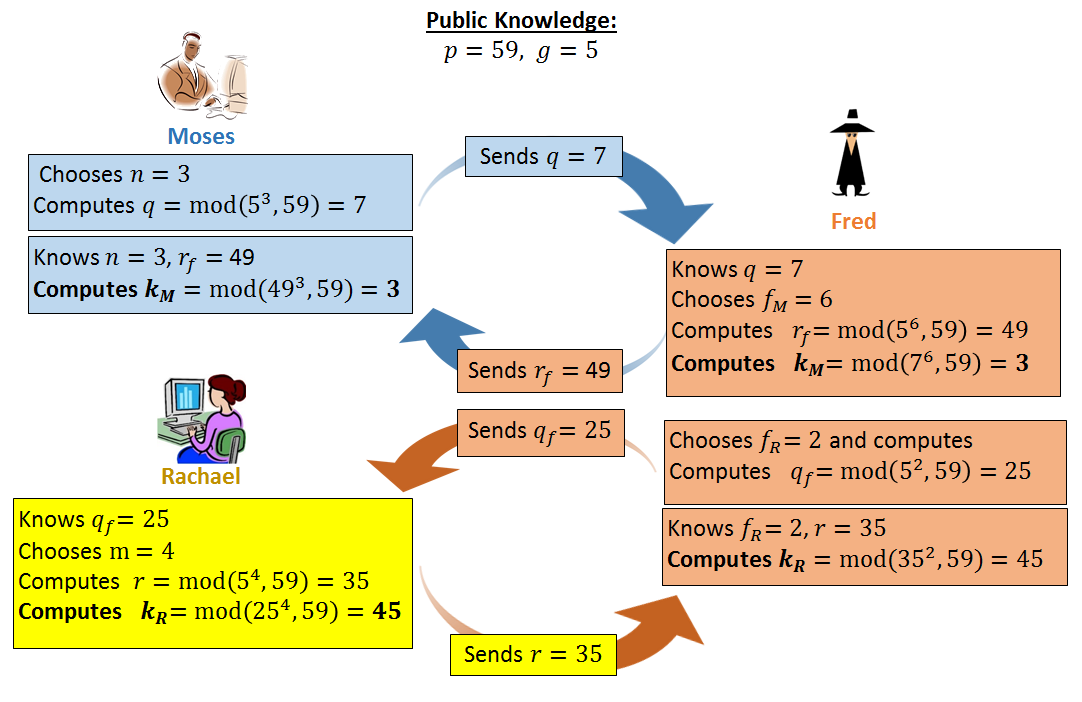
\includegraphics[width=5in]
	         {images/DHKE_18.png}}
	  \caption{\label{fig:DH:DHKE_2} MiM Attack during Moses and Rachael's Key Exchange }
\end{figure}

Following Figure~\ref{fig:DH:DHKE_2}, Fred establishes a shared key $k_M$ with Moses and another secret key $k_R$ with Rachael.  Now Moses thinks $r_f$ is Rachael's public key, and Rachael thinks that she has Moses' public key. Moses and Rachael both combine their private keys with Fred's public keys and create two different symmetric keys, $k_M$ and $k_R$ respectively. At this point if Moses or Rachael sends a message then Fred is free to decrypt and encrypt the message using the appropriate symmetric key. 

\begin{exercise}{}
Redo Figure~\ref{fig:DH:DHKE_2} using different values of $p, g, n,m, f_n,$ and $f_m$, remember to choose a prime for $p$ and a primitive root for $g$ (there are many primitive root calculators you can find online).
\end{exercise}

\begin{exercise}{}
Replace all the numbers in the formulas found in Figure~\ref{fig:DH:DHKE_2} with letters, as seen in Figure~\ref{fig:DH:DHKE_1}.
\end{exercise}

\begin{exercise}{}
Given $p=73,$ and $g=11$ find $q, r, r_f, q_f, k_M,$ and $k_R$ if Moses chooses $n=5$, Rachael chooses $m=4$ and Fred chooses $f_M=3$ and $f_R=2$.
%ans:q=13, k_M=7, r_f=17, q_f=48, r=41, k_R=2
\end{exercise}

DHKE is vulnerable to this type of MiM attack since Moses cannot verify that Rachael was the originator of the message, and vice-versa.  Fortunately, you can prevent a MiM attack by using a \term{digital signature}.  To understand what a digital signature does, first let us consider the purpose of a conventional signature.  Typically, a signature is uniquely scribed on a document, and is proof of authentication.  Comparitively, a digital signature is intended to authenticate the origin of the sender and ensure the integrity of the message.  In Section \ref{sec:DHKE:1}, we described how to verify messages by using a private key to encrypt and a public key to decrypt.  Once a message is signed and encrypted, it cannot be altered without destroying the signature which authenticates the message. In summation, the MiM can prevent Moses and Rachael from establishing a shared key (by tampering with the message), but Fred cannot eavesdrop on any secret communication.

 Diffie-Hellman is just one of many key exchange algorithms you can use. In the next section, we will talk about a different way to exchange keys that is even more secure.

\section{Elliptic curve cryptography}\label{sec:ECC:2}

In the previous section we saw that the longer the key, the greater the security. The disadvantage to long keys is they require sending more information, thus slowing down communication.  Elliptic curve cryptography (ECC) is one approach to the public key sharing dilemma that offers greater security with smaller keys. The table in Figure~\ref{fig:DH:DHKE_9} shows the relationship between key length and security for three different cryptosystems: RSA, Diffie-Hellman, and ECC.  In the table, 'key length' refers to the number of binary bits in the key: for comparison, a 160 bit key has 49 decimal digits, while a 1024 bit key has 309 decimal digits. The 'security level' is also measured in bits (80, 128, 192, 256) where these bits refer to the size of the number of computational steps necessary to break the code.  For example, a security level of 80 means that $2^{80}$ computations are required to break the code (from reference(\ref{Certicom})). To give you an idea of what this means practically, in 2002 it took $10,000$ computers (mainly PCs) running 24 hours a day for 549 days to break an ECC system with a 109 bit key length. A 160-bit ECC would be $2^{25}$ times more secure: which means that (with 2002 technology) it would take one billion computers over 500 years to crack it.
\begin{figure} [H]
	   \center{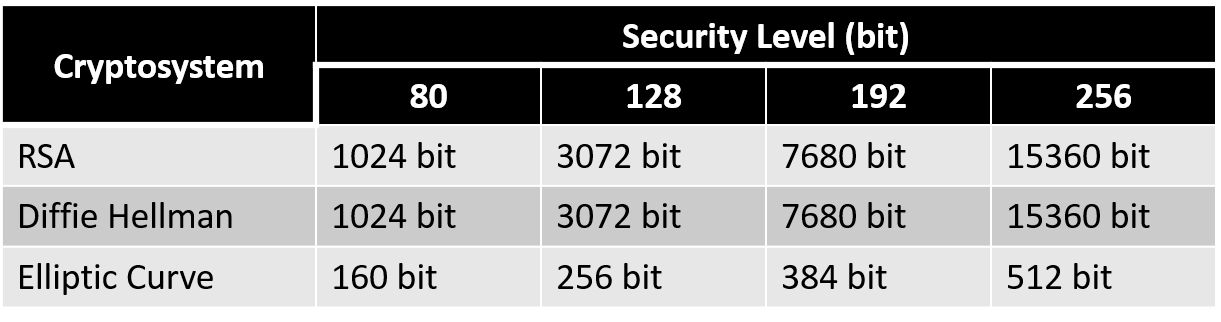
\includegraphics[width=5in]
	         {images/DHKE_9.png}}
	  \caption{\label{fig:DH:DHKE_9}Key bit lengths of cryptosystems for different security levels recommended by the National Institute of Standards and Technology, (from reference (\ref{mobile}))}
\end{figure}
Referencing the table in Figure~\ref{fig:DH:DHKE_9}, we can see that an ECC cryptosystem with a 160 bit key has a similar security level to RSA and Diffie-Hellman with 1024-bit keys. This means the same security with 6 times less information--a significant difference! 

\begin{exercise}{}
How long would it take to crack a cryptosystem with a 128 bit security, using a billion modern computers with 2 GHz processors?
\end{exercise}

Now that we have established the benefits of ECC, let us see what elliptic curves are all about. Our discussion will be quite wide-ranging, and touch on several areas of mathematics. Although we will not go into the background, elliptic curves originally arose from complications using calculus. Elliptic curves also have deep connections to the theory of complex functions. 

\subsection{Definition of elliptic curves}
An Elliptic Curve (EC) is the set of solutions $(x,y)$ of  an equation of the form $y^2 = x^3 + ax + b$, where $a$ and $b$ are real coefficients.  See Figure~\ref{fig:DH:DHKE_5} below for graphs of some elliptic  curves.  
\begin{figure}[htbp]
	   \center{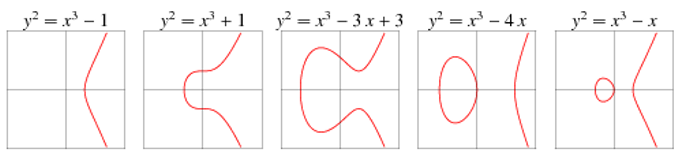
\includegraphics[width=5in]
	         {images/DHKE_5.png}}
	  \caption{\label{fig:DH:DHKE_5}  Geometric shapes of elliptic curves, (from reference (\ref{Wolframalpha}))}
\end{figure}
Additionally, ECs are not allowed to have double or triple roots.  A triple root produces a cusp in the graph, and a double root produces a self-intersection (see graphs in Figure~\ref{fig:DH:DHKE_10}). See graphs in Figure~\ref{fig:DH:DHKE_10} for examples of elliptic curves with double and triple roots.
\begin{figure}[htbp]
	   \center{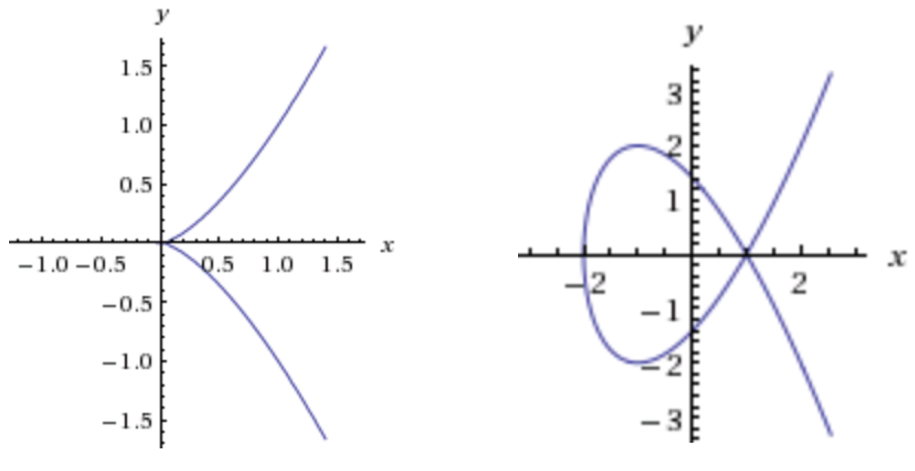
\includegraphics[width=3in]
	         {images/DHKE_10.png}}
	  \caption{\label{fig:DH:DHKE_10}(Left) E: $ y^2$ = $x^3$ and (Right) E: $ y^2$ = $x^3-3x+2$, (From reference (\ref{Corbellini})}
\end{figure}
 It turns out that we can guarantee that the EC has no double or triple roots if the coefficients $a$ and $b$ satisfy the following equation: $4a^3 + 27b^2 \neq 0$. 

\begin{exercise}{dubroots}
		\begin{enumerate}[(a)] 
	\item  Prove that if the equation $y^2 = x^3 + ax + b$ has a double or triple root, then $4a^3+27b^2=0$. 
\hyperref[sec:further_crypt:hints]{(*Hint*)}
	\item Prove the converse to part (a), that is show that if $4a^3 + 27b ^2=0$, then the equation has a double or triple root. \hyperref[sec:further_crypt:hints]{(*Hint*)}
\end {enumerate} 
\end{exercise}

All of the cryptosystems that we have studied so far have been based on group operations associated with a particular group. For example, Diffie-Hellman used discrete exponentiation (which is repeated multiplication in $U(p)$) to construct a one-way function. In order to make use of elliptic curves to construct cryptosystems, we will need to show that we can associate a group with each elliptic curve. In the following sections, we will show first how to define an arithmetic operation on the points of  any  elliptic curve: and then that this operation is in fact a group operation.

\subsection{Elliptic curve arithmetic}\label{sec:ECA}
In this section, we show how to do arithmetic on elliptic curves. Specifically, we define an operation (denoted by `+') which acts on two points of an elliptic curve, to give another point on the same curve. 

Suppose that $P_1$ and $P_2$ are two points on an EC. We will consider first the case where $P_1 \neq P_2$: later we will consider the case where  $P_1= P_2$. Geometrically, if the two points are different then $P_1 + P_2$ is given by drawing a line from point $P_1$ to point $P_2$ and continuing the line until it intersects the elliptic curve, then reflect that point about the $x$-axis.  See Figure~\ref{fig:DH:DHKE_6} for a geometric representation of the operation $P_1+P_2$.

\begin{figure}[htbp]
	   \center{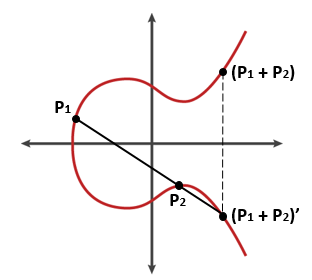
\includegraphics[width=2.5in]
	         {images/DHKE_6.png}}
	  \caption{\label{fig:DH:DHKE_6}Adding two distinct points, $P_1 + P_2$ on the EC (from reference (\ref{wikipedia2017})).}
\end{figure}

It turns out that $P_1 + P_2$ is always defined on the EC (except in one special case which we will explain a little bit later), even though sometimes the result of $P_1 + P_2$ is quite far away from both $P_1$ and $P_2$.  For instance, take E: $ y^2$ = $x^3 - x$, and points $P_1 = (2, \sqrt{6})$ and $P_2 = (3, -\sqrt{24})$.  Then $P_1 + P_2 = (49,342.93)$ (we'll show this later in Example \ref{example:further_crypt:find P3}), as illustrated in Figure~\ref{fig:DH:DHKE_16}. 
\begin{figure}[htbp]
	   \center{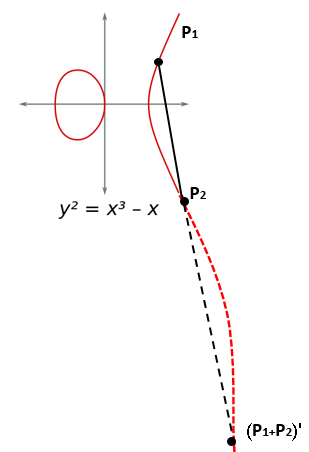
\includegraphics[width=2in]
	         {images/DHKE_16.png}}
	  \caption{\label{fig:DH:DHKE_16} $P_1 + P_2$ is always defined on the EC (from reference (\ref{wikipedia2017})).}
\end{figure}

\begin{example}{ec:realplus}
Given E: $y^2 = x^3 + ax + b$, $P_1 = (x_1, y_1)$, $P_2 = (x_2, y_2)$, and $P_3 = (x_3, y_3)$. Find $P_3$, where $ P_3 =  P_1 + P_2$.

\noindent
The steps of this calculation are as follows:
\begin{enumerate}[(a)]
\item
Compute the slope of the line $m$ through $P_1$ and $P_2$ as follows:  \[ m =(y_2 - y_1) \cdot (x_2- x_1)^{-1}, \text{for } P_1 \neq P_2  \] 
\item
Use the point-slope formula $y - y_1 = m(x-x_1)$  in order to find equation of the line that passes through the two points.  Rewrite as: \[y  = m(x-x_1) + y_1\]
\item
It turns out that the sum of the roots is $m^2$ (see Exercise~\ref{exercise:further_crypt:root3}). So we have
\[x_1 + x_2 + x_3 = m^2, \text{ which implies } x_3 =   m^2 -  x_1 - x_2.\]
\item  The third point of intersection is $(x_3, -y_3)$. So  we may plug $x_3$ into $(-y_3)  = m(x_3-x_1) + y_1$ to obtain $y_3$. 
\item Finished!  $P_3 = (x_3,y_3)$.
\end{enumerate}
 \end{example} 

\begin{exercise}{root3}
In part (c) of Example~\ref{example:further_crypt:ec:realplus} we mentioned that $x_1+x_2+x_3=m^2$, where $x_1,x_2,x_3$ are the x-coordinates of three intersections of the a with the EC and $m$ is the slope of the line.  In this exercise, we will prove this.
\begin{enumerate}[(a)]
\item
Substitute the equation for $y$ in (b) into equation E. The resulting equation can be rearranged to form a cubic equation in $x$ of the form: $0 = x^3 + c_2 x^2 + c_1 x + c_0$, where $c_1, c_2, c_3$ depend on the parameters $a,b,m,x_1,x_2$. Find the coefficient $c_2$ in terms of these parameters.
\item
The cubic equation $0 = x^3 + c_2 x^2 + c_1 x + c_0$ has three roots, so the cubic equation can be factored:  $x^3 + c_2 x^2 + c_1 x + c_0 = (x-x_1)(x-x_2)(x-x_3)$. Use this equality to express $c_2$ in terms of $x_1, x_2, x_3$.
\item
Based on your results in (a) and (b), show that $m^2 = x_1 + x_2 + x_3$.
\end{enumerate}
\end{exercise}

\begin{example}{} 
Given E: $y^2 = x^3 - 2x$, $P_1 = (0,0)$, $P_2 = (-1,1)$, Find $P_3=P_1 + P_2$.
		
\begin{enumerate}[(a)]
\item
Slope :
$ m =(1 - 0) \cdot (-1- 0)^{-1}=-1$.
\item
Equation of line:	$y - 0 = -1(x- 0)$ or $y =-x $.
\item
Use $x_3 = m^2 - x_1 - x_2$ to obtain: $x_3 = (-1)^2 - 0 - (-1) = 2$.
\item
Use equation of line with $y=-y_3$ and $x=x_3$:  $-y_3 = -2$ or $y_3=2$.
\item
$P_3 = (2,2)$.
\end{enumerate}
\end{example}
\begin{example}{find P3} Given E: $y^2 = x^3 - x$, $P_1 = (2, \sqrt{6})$, $P_2 = (3, -\sqrt{24})$ from Figure~\ref{fig:DH:DHKE_16} above.
	Find $P_3$, where $P_3 = P_1 + P_2$.
\begin{enumerate}[(a)]
\item 
Slope: $m =( -\sqrt{24}-\sqrt{6})$ $\cdot$ $(3-2)^{-1} = -3\sqrt{6}  $ \\
\item
Line: $y + \sqrt{24} = -3\sqrt{6}(x - 3)$, which simplifies to $y = -3\sqrt{6}x + 7\sqrt{6}$.
\item 
Use $x_3 = m^2 - x_1 - x_2$ to obtain: $x_3 = (-3\sqrt{6})^2 - 2 - 3 = 49$.
\item
Plug $(1,-y_3)$ in for $(x,y)$ in the equation for the line: $-y_3 = -3\sqrt{6}\cdot 49+7 \sqrt{6}$, which implies $y_3 = 140\sqrt{6}$. 
\item
$P_3 = (49,140\sqrt{6}) \approx (49,342.93)$.
\end {enumerate}  
\end{example}

\begin{exercise}{} Given E: $y^2 = x^3 - 2x$, $P_1 = (2, 2)$, $P_2 = (-1, 1)$, find $P_3$, where $P_3 = P_1 + P_2$.
\end{exercise}

\begin{exercise}{} Given E: $y^2 = x^3 - x + 1$, $P_1 = (3, 5)$, $P_2 = (1, 1)$, find $P_3$, where $P_3 = P_1 + P_2$.
\end{exercise}

If the two points are the same, $P_1 = P_2 = (x_1,y_1)$, then a tangent line to the point is drawn and the point of intersection to the EC is then reflected about the x-axis.  This is often referred to as \term{point doubling}\index{Point doubling! in elliptic curves}. The slope for this line is, 
\[m = (3x_1^2 + a) \cdot (2y_1)^{-1},\] 
which may be found using implicit differentiation (note that $a$ refers to the coefficient of $x$ in the elliptic curve equation--see Example~\ref{example:further_crypt:ec:realplus}).  See Figure~\ref{fig:DH:DHKE_7} below for a geometrical representation of point doubling.

\begin{exercise}{}
Derive the equation for $m$ by taking the derivative of E and solving for $\frac{dy}{dx}$. Show your steps.
\end{exercise}

In the case of point doubling, once $m$ is found the expression for  the $x$ coordinate of the other intersection of the tangent line with the curve is:
\[ x_3 = m^2 - x_1 - x_1\]
(this is because $x_1$ is a double root of the cubic expression which gives the x-coordinates of the intersections between the EC and the tangent line). Once we have $x_3$, then we may find $y_3$ as before:
\[ -y_3 = m(x_3-x_1) + y_1 \]
and $2P_1$ is given by $(x_3,y_3)$.

\begin{figure}[htbp]
	   \center{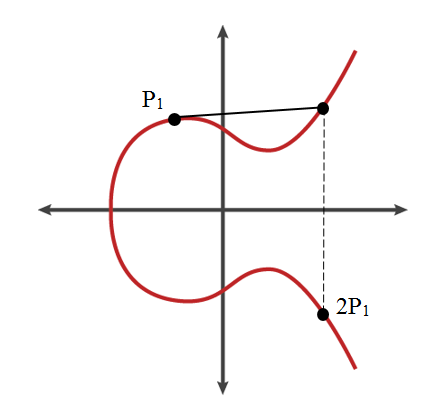
\includegraphics[width=2.5in]
	         {images/DHKE_7.png}}
	  \caption{\label{fig:DH:DHKE_7}Point doubling on the EC (from reference (\ref{Corbellini})).}
\end{figure}
There is one scenario where addition of two points doesn't give a point on the curve. Given a point $P$, we define  $-P$ as the reflection of $P$ about the x axis: so  if $P = (x, y)$, then $-P = (x, -y)$. The line through $P$ and $-P$ is vertical, and does not intersect the curve at any other point.  In order to make addition well-defined in this case we may create a notional \term{point at infinity}. See Figure~\ref{fig:DH:DHKE_19} below for a geometrical representation of the point at infinity.
\begin{figure}[htbp]
	   \center{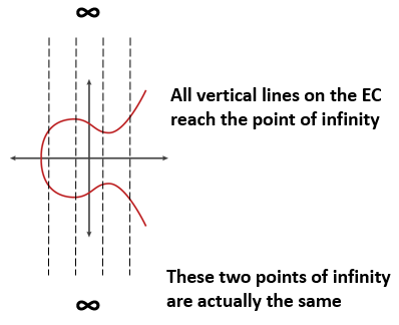
\includegraphics[width=3.5in]
	         {images/DHKE_19.png}}
	  \caption{\label{fig:DH:DHKE_19}The point at infinity located at $(0,\infty)$ (from reference (\ref{wikipedia2017})).}
\end{figure}
The point at infinity can be thought of as located at the point $(0,\infty)$, so that the line through any point $(x, y)$ and the point at infinity is a vertical line with infinite slope. Additionally, the point at infinity is its own reflection, so we consider $(0,\infty)$ and $(0,-\infty)$ as a single point, which we denote by the symbol $\infty$. You may think of the y  axis ``wrapping around'' so that when you keep moving in the +y direction eventually you wrap around to the -y axis.
\subsection{Elliptic curve groups}
Remarkably, it turns out that the `+' operation turns the elliptic curve (plus the point at infinity)  into a group.  In this section we'll verify all of the group properties. 

\begin{enumerate}[1.]
\item \textbf{Identity}: The point at infinity serves as the identity element.  The line connecting $\infty$ with $P$ intersects $-P$, so its reflection about the x-axis is $P$. Therefore, $P + \infty = P$ and $\infty + P = P$. 
\begin{figure}[htbp]
	   \center{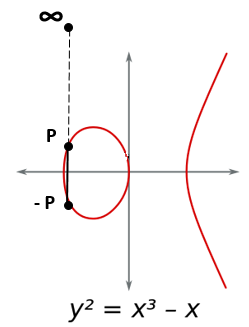
\includegraphics[width=2in]
	         {images/DHKE_13.png}}
	  \caption{\label{fig:DH:DHKE_13} Identity property for EC: $\infty + P = P + \infty = P$ (from reference (\ref{wikipedia2017})).}
\end{figure}
\item \textbf{Inverse}: A line through $P$ and$-P$ goes through $\infty$, and $\infty$ is its own reflection (see Figure \ref{fig:DH:DHKE_13}). Another way of saying this is, $P + (- P) = \infty$. In the same way, we can show that $(-P) + P = \infty$. Therefore the inverse of $P$ is $-P$. 

\item \textbf{Closure}: if $P_1$ and $P_2$ are points on the elliptic curve then $P_1 + P_2$ is also a point on the curve; as stated (without proof) in Section \ref{sec:ECA}.
\item \textbf{Associativity}:$(P_1 + P_2) + P_3 = P_1 + (P_2 + P_3)$. This is always true (for an example, see Figure~\ref{fig:DH:DHKE_12} below),  but it is not at all easy to prove. See for example \url{math.rice.edu/~friedl/papers/AAELLIPTIC.PDF}, which gives a 5-page ``elementary'' proof.
\begin{figure}[htbp]
	   \center{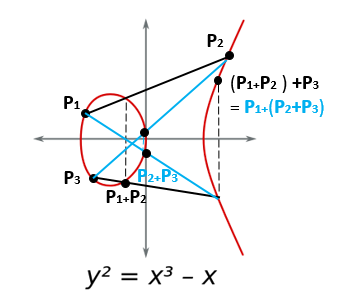
\includegraphics[width=2.5in]
	         {images/DHKE_12.png}}
	  \caption{\label{fig:DH:DHKE_12} Associative property for EC (from reference (\ref{wikipedia2017})).}
\end{figure}
\end{enumerate}

These properties are sufficient to establish the fact that the `+' operation on an elliptic curve defines a group.

\begin{exercise}{}
Does the '+' operation define an Abelian group? Prove your answer.
\end {exercise}

\subsection{Elliptic curves over $\mathbb{Z}_p$}\label{sec:ECA2} 

Thus far we have looked at elliptic curves whose coefficients are real numbers. Unfortunately, computer calculations with real numbers are prone to rounding errors, so real number arithmetic is not suitable for modern cryptography. To avoid this problem,  instead of using real numbers we use \emph{finite fields}\index{Finite fields!in EC cryptography}, which are finite additive groups that also have a multiplication operation with inverse. The simplest finite fields are  $\mathbb{Z}_p$ (integers mod $p$),  where $p$ is prime. In this section we will demonstrate how to do arithmetic with elliptic curves over $\mathbb{Z}_p$.

At the end of the previous section, we showed that our new  `+' operation allows us to define a group on the set of points of an elliptic curve, when the curve is a subset of $R^2$ and is defined using real coefficients.  It turns out that exactly the same argument can be used to show the very same group property for curves with coefficients in $\mathbb{Z}_p$, which are subsets of $\mathbb{Z}_p \times \mathbb{Z}_p$.  

We saw in Section \ref{CyclicSubgroups} that every element of a group defines a \term{cyclic subgroup}\index{Cyclic subgroup! in EC cryptography}. Specifically, if the group $G$ is finite, then for any element $g \in G$ the set 
\[ {\var id}, g, g^2, g^3, \ldots, g^{n-1} \ \]
is a subgroup of $G$, where $n$ is the \emph{order} of $g$ and satisfies $g^n = {\var id}$. In EC cryptography, extensive use is made of cyclic subgroups.  Any EC cyptosystem is based on a single group element, which is referred to as a \term{generator}\index{Generator! in EC cryptography}.  In practice, the generator is added to itself repeatedly. Follow the examples below to see how this works.

\emph{Note} that in the following examples we will use `+'  and `$\cdot$' to denote addition and multiplication in the particular  $\mathbb{Z}_p$ that we are working with: in other words, `+' and `$\cdot$' in the following are the same as `$\oplus$' and `$\odot$' which we used in Chapter~\ref{modular}  (it's simpler to write this way, and this is how it's done in most references.) You'll have to pay attention to what `+' is operating on in order to discern its meaning:  for example, in the expression $P+P$ we're referring to the elliptic curve operation defined in the previous section, while in the polynomial $x^3 + 2x + 2$  the `+' refers to modular addition. 

\begin{example}{P1+P2} In this example we'll use arithmetic mod 17, so  all coefficients and variables take values on $\mathbb{Z}_{17}$.  

Given E: $y^2 = x^3 + 2x + 2$, and $P = (5,1)$,  we want to find $2P$, where $2P = P + P$.\\ \\
First we use the slope of the tangent line, using the same formula we did for the real case in Example \ref{example:further_crypt:ec:realplus}:	
\[m = (3x_1^2 + a) \cdot (2y_1)^{-1}\]	
We may then calculate (remember we're doing arithmetic in  $\mathbb{Z}_{17}$!)
\begin{align*}
		m &\equiv ( (3 \cdot 5^2) + 2) \cdot (2 \cdot 1)^{-1} \\
	          &\equiv  (77) \cdot (2)^{-1} \\
                     &\equiv (9) \cdot (9)\\
                     &\equiv 81 \\
                    &\equiv 13 \pmod{17}
		\end{align*}
Next we use the following formulas (which we used before for reall elliptic curves) to find $x_3$ and $y_3$: \[ x_3 = m^2 - 2x_1  , \text{and~} y_3 =-(  m(x_3 - x_1)+y_1)\]
where once again, arithmetic is in $\mathbb{Z}_{17}$:
\begin{align*}
		x_3 &\equiv  (13^2 - 5 - 5 ) \\
	          &\equiv 159\\
                     &\equiv 6 \pmod{17}
		\end{align*}
			\begin{align*}
		y_3 &\equiv - (13(6 - 5) +1) \\
	          &\equiv -14\\
                     &\equiv 3 \pmod{17}
		\end{align*}
Therefore, $2P = (6,3)$.
\end{example}
\begin{exercise}{P}
Using the equations from Example~\ref{example:further_crypt:ec:realplus} parts (c) and (d), find the following: $3P, 4P, 5P, ..., 20P.$  Note that $3P = 2P + P,  4P = 3P +P,$ and so on. Note also that arithmetic operations are to be performed in mod 17.  What do you notice about $18P,  19P,$ and $20P?$
\end{exercise}
In view of what we have just discussed, let's reconsider the Diffie-Hellman Key Exchange which we described in Section~\ref{sec:DHKE:1}. A little thought should convince you that in that section we made use of cyclic subgroups as well. So using Example \ref{example:further_crypt:P1+P2} and Exercise~\ref{exercise:further_crypt:P}, let's revise the Diffie-Hellman Key Exchange, but this time we'll use the cyclic group associated with the elliptic curve.  Use Figure~\ref{fig:DH:DHKE_8} as a guide to help you answer the following exercise.

\begin{figure}[htbp]
	   \center{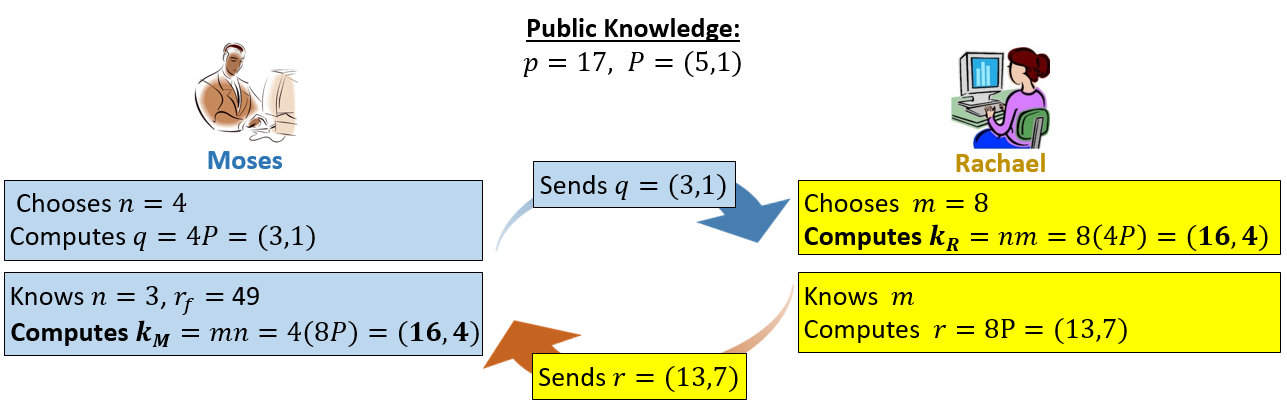
\includegraphics[width=5in]
	         {images/DHKE_8.png}}
	  \caption{\label{fig:DH:DHKE_8} Elliptic Curve Key Exchange between Moses and Rachael }
\end{figure}

\begin{exer}
Using Example \ref{example:further_crypt:P1+P2} and Exercise~\ref{exercise:further_crypt:P}, what is the shared key exchange if Moses chooses $n = 9$ and Rachael chooses $m = 3$?
\end{exer}
\subsection{An encryption system using elliptic curves} 
In Chapter \ref{crypt} we explained how to use RSA with a shared key to exchange secret messages.  We can construct a similar cryptosystem on the basis of elliptic curves. In this section, we'll describe one way that this may be done. The following discussion is a simplified version of reference (\ref{Kumar}).

Suppose Moses and Rachael would like to communicate a message using ECC, then they should first agree upon an elliptic curve and a code table. Each character of the encrypted message will correspond to a point on the elliptic curve.

Next, Rachael and Moses construct public and private keys as follows. First, Rachael and Moses agree upon an elliptic curve, modulus, and a random point $C$ on the EC: in general, this will be public knowledge.  Additionally, Rachael selects at  random a large positive integer $\alpha$ which is  Rachael's private key. She computes $A = \alpha C$ which is her public key (recall that $\alpha C$ denotes adding the point $C$ $\alpha$ times, using EC addition). Moses similarly takes a large positive integer $\beta$ as his private key, and computes $B = \beta C$ as his public key.

Now if Moses wants to encrypt a message, he may do so one character at a time as follows. Suppose the character that he wants to encrypt corresponds to the point $M$ on the elliptic curve.   He chooses a random number $\gamma$ (which will be different for each character in the message). He then computes:
\[
E_1=\gamma C \text{   and   }
E_2 = M +  \gamma A. 
\]
Moses then communicates $E_1$ and $E_2$ to  Rachael.  After receiving this information, Rachael may decrypt the message by computing $E_2 - \alpha E_1$.

\begin{exercise}{}
\begin{enumerate}[a]
\item
Show that by computing $E_2 - \alpha E_1$, Rachael will correctly recover  the character $M$.
\item
Suppose a third party knows $E_1, E_2, A,$ and $C$. What else would a third party have to find out in order to obtain $M$?  Explain why it is difficult for the third party to gain this knowledge.
\end{enumerate}
\end{exercise}

\begin{exercise}{}
\begin{enumerate}[a]
\item
Suppose Rachael wants to send a character to Moses.  What information should she send?
\item
What equation should Moses use to decode the information from Rachael?
\end{enumerate}
\end{exercise}

To see how this works in practice, let's consider a simple example (reader beware: the modulus is way too small to make this a practical cryptosystem). We will consider the elliptic curve in $Z_{37}$ $\times$ $Z_{37}$ given by the equation $y^2 = x^3 + 2x + 9$ which is shown in Figure~\ref{fig:DH:DHKE_11} below. Notice how the graph of the function using modular arithmetic is a collection of discrete points on the curve rather than based on a continuous graph like the elliptic curves over the real numbers.

\begin{figure}[htbp]
	   \center{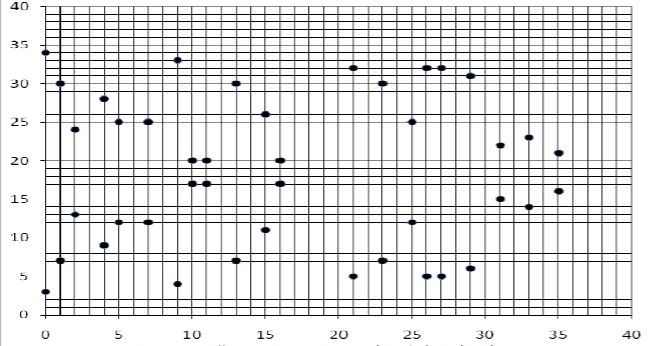
\includegraphics[width=5in]
	         {images/DHKE_11.png}}
	  \caption{\label{fig:DH:DHKE_11} Elliptic Curve, $(y^2 = x^3 + 2x + 9)$ in $Z_{37}$ x $Z_{37}$, (from reference (\ref{Kumar}))}
\end{figure}

In order to encode letters and numbers, we first need to assign different characters to different points on the curve. The table in Figure~\ref{fig:DH:DHKE_17} gives the character assignment that we'll use. Notice the order of points in the table: we start with (5,25), then the second number $(1,30) =(5,25)+(5,25)$, the third number $(21,32)=(5,25)+(5,25)+(5,25)=3(5,25)$, and so on. This table is public, known to everyone. Note that in the case of a very large modulus, there is no difficulty in assigning a single character to multiple points on the curve, as long as each point has no more than one character assigned to it.

\begin{figure}[htbp]
	   \center{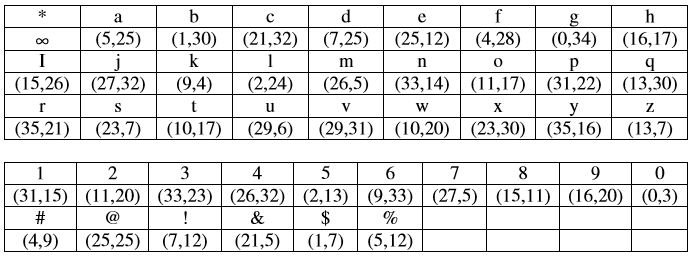
\includegraphics[width=5.25in]
	         {images/DHKE_17.png}}
	  \caption{\label{fig:DH:DHKE_17} Code table using the EC agreed upon by Moses and Rachael, (from reference (\ref{Kumar}))}
\end{figure}


\begin{example}{26} Moses will send the message, ``attack" using the code table above. The point $C$ is chosen as $(9,4)$. 

First, Rachael must establish her private and public key (Moses doesn't have to, because he's only sending and not receiving). Rachael chooses $\alpha= 5$, so that $A = 5C = 5(9,4)$. In this simple case, we  may use  the table in Figure~\ref{fig:DH:DHKE_17} to facilitate the calculation of $A$.  Notice that the point $C=(9,4)$ is the $11^{\textrm{th}}$ point in the table (counting $\infty$ as the zeroth point, (5,25) as the first point, (1,30) as the second point, etc). This means that $C = 11(5,25)$, and thus $5C = 5\cdot11(5,25) = 55(5,25)$.  However the point $(5,25)$ generates a cyclic group of order 37, and $\mod(55,37)=18$, so $55(5,25)=18(5,25)$.  The $18^{\textrm{th}}$ entry in the table is (31,15), which is Rachael's public key $A$.

Now Moses must encrypt his message one character at a time. The first character of ``attack'' is ``a'', which according to the table corresponds to $M=(5,25)$.  Let's suppose that Moses chooses $\gamma = 8$ for this character. We thus obtain:
\[
E_1=\gamma C = 8(9,4)=(33,14)  \text{   and   } 
E_2 = M +  \gamma A=(5,25) + 8(31,15) = (15,11). 
\]

Thus Moses should send the pair of points $(33,14)$ and $(15,11)$ to Rachael. Since $(33,14)$ and $(15,11)$ are the $18^{\textrm{th}}$ and $34^{\textrm{th}}$ entries of the table respectively, it's easier for him simply to send the numbers 18 and 34, because Rachael can easily recover the points from these numbers.

\begin{exercise}{}
\begin{enumerate}[a]
\item
Verify the values of $E_1$ and $E_2$ computed above. Show your calculation.
\item
Verify that using these values of $E_1$ and $E_2$ and $\alpha=5$, Rachael can correctly decode the character.
\end{enumerate}
\end{exercise}

\begin{exercise}{}
To encode t, t, a, c, k Moses chooses $\gamma = 12,19,2,3,23$ respectively. 
\begin{enumerate}[a]
\item Give the 5 pairs of numbers that Moses sends as cyphertext
\item Verify that Rachael decodes each pair of numbers correctly.
\end{enumerate}
\end{exercise}

\end{example}

\subsection{Next steps}
The examples we've given show the basic idea of ECC, but genuinely practical ECC systems are somewhat more complicated. Notice the progression from Section~\ref{sec:ECA} to \label{sec:ECA2}. We first introduced elliptic curves as solution sets in $\mathbb{R}^2$ for a certain type of polynomial equation. But we then remarked that unfortunately these curves are not suitable for practical cryptography, because computers have trouble with real numbers. So in the next section we looked at elliptic curves that are subsets of $\mathbb{Z}_p \times \mathbb{Z}_p$ where $p$ is a prime, as in Figure~\ref{fig:DH:DHKE_11}. But there are disadvantages to $\mathbb{Z}_p$ as well: finding enormous primes is not all that easy. It turns out there is yet another alternative for sets for elliptic curves to live in:  these sets are called \term{Galois Fields}. Galois fields are derived from polynomials, where the polynomials have coefficients in $\mathbb{Z}_p$ (in practice, usually $p=2$).  Since we haven't really looked into polynomials yet, we're not quite ready to dive into this aspect of ECC just yet.  So, you have something to look forward to! 

%In practice, it is important to choose a large prime number $p$, in order to make it difficult for an eavesdropper to crack your code.  Internet protocols usually use a minimum of a 1024-bit prime number for $p$, which is equivalent to $2^{1024}$ or roughly 300 decimal digits long.  So, there are $2^{1023}$ different possibilities for 1024 bits (where the highest bit is a `1'). It is not necessary to generate your own prime.  There are many records of large primes published that can be referenced. For example, if you visit \url{http://primes.utm.edu/} you can see some lists of 210 digit primes and larger (from reference (\ref{Caldwell})).
%
%\subsection{Galois Field} 
%As a review, there are three types of algebraic structures: groups, rings, and fields (see Figure~\ref{fig:DH:DHKE_3}); each structure building from the previous structure.  Each structure is defined as a set of elements where: the given operation is closed, has the identity element, has the inverse element, and is associative. For the purpose of this text we'll focus on Finite Fields (FF), which is a field that contains a finite number of elements and is also known as Galois Fields (GF). Applications of Galois Fields can be seen in CD players, DVD players, disk storage systems, and apps found on computers, tablets and smart phones.
%\begin{figure}[htbp]
%	   \center{\includegraphics[width=4.5in]
%	         {images/DHKE_3.png}}
%	  \caption{\label{fig:DH:DHKE_3} Algebraic structures and types of FFs }
%\end{figure}
% GFs only exist if they have $P^m$ elements, $GF(P^m)$. So, there is a GF with 27 elements $GF(27) = GF(3^3)$, there is a $GF$ with 256 elements $GF(256) = GF(2^8)$, etc.  In EC we are interested in Binary Fields (BFs), GFs of order $2^m$, with $m \geq 1$.  Operations in the BF are defined in terms of an irreducible polynomial with degree $m$, this polynomial is also referred to as the reduction polynomial.  This means that the binary polynomial cannot be factored as a product of binary polynomials of degree less than $m$.  There are always $2^m$ elements in $GF(2^m)$.
%
%\begin{rem} Given the polynomials $a,b \in  GF(P) = (0,1,2,...,P-1)$ then 
%\begin{align*} 		
%		a + b &\equiv c (\bmod P)\\
%		a - b &\equiv d (\bmod P)\\
%		a \cdot b &\equiv e (\bmod P) \quad \text{ ,the multiplicative group does not include 0}\\
%		a^{-1} &\equiv b, \mathrm{~if~} \bmod (ab, P) = 1
%\end{align*}
%\end{rem}
%\begin{eg} Below are the 8 elements of $GF(2^3)$:
%\begin{align*}
%0, \quad 1, \quad X, \quad X +1, \quad X^2, \quad X^2+1, \quad X^2 + X, \quad X^2 + X + 1
% \end{align*}
%\text{Adding two polynomials in $GF(2^3)$ is as follows:}
%\begin{align*}
%	f(x) &= X^2 + X\\
%	g(x) &= X^2  + 1\\
%           f(x) + g(x) &= X  + 1
% \end{align*}
% \text{Notice that the addition of the coefficient $X^2$ and the constant 1 = 0 in GF($2^3$). Also, it is }
%\text{important to note that the binary field has only two coefficients (0,1) so subtraction and}
%\text{addition are the same.}
%\end{eg}
%\begin{exer} Given $GF(2^4)$, add the following two polynomials:
%\begin{align*}
%	f(x) &= X^3 + X^2 + X + 1\\
%	g(x) &= X^2  + 1
% \end{align*}
%\end{exer}
%
%\begin{exer} Given $GF(2^8)$, subtract the following two polynomials, $f(x) - g(x)$:
%\begin{align*}	
%	f(x) &= X^8 +         X^6 +          X^3 + X^2 + 1\\
%	g(x) &=        X^7 + X^6 + X^5 +          X^2
%\end{align*}
%\end{exer}
%Next let us discuss polynomial multiplication and the problem it presents. To multiply two polynomials, multiply each term in one polynomial by each term in the other polynomial. The problem with this is that it gives you polynomials whose degree is too large. When this happens you have to use some method to reduce the degree. This method is similar to the method we used to construct modular addition in the first place.  In modular addition mod p, to define multiplication and then take the remainder mod p.  In Galois fields we multiply the two polynomials and then take the remainder after division by a fixed polynomial which is called the \term{reduction polynomial}.  The reduction polynomial plays the same role as the number $p$ in $\mathbb{Z}_p$.
%
%\begin{eg} Given $GF(2^4)$ and the reduction polynomial $X^4 + X + 1$, then multiplying two polynomials is as follows:
%\begin{align*}	
%	f(x) &=  X^2 + X + 1\\
%	g(x) &= X^3 + 1\\
% f(x) \cdot g(x) &= X^5 + X^4 + X^3 + X^2 + X + 1 (\bmod X^4 + X + 1)\\ 
%	       &= - X^3 + X \text{ , is the remainder (see below for explanation) }
%\end{align*}
%\begin{center}
%\begin{tabular}{rrcrcrcrcrcr}
%        &  $x$  &  $+$  &      $1$         \\ \cline{2-12}
% \multicolumn{1}{r|}{$x^4 + x + 1$}
%        &  $x^5$  &  $+$  &  $x^4$  &  $+$  & $ x^3$  &  $+$  &  $x^2$  &  $+$  & $ x$  &  $+$  &  $1$  \\
%        & $x^5$   &  $+$  &       	&          &      	  &          &  $x^2$   & $+$  &  $x$     \\ \cline{2-12}
%        &         &       &         $x^4$  & $+$   &  $ x^3$  &   $+$  &             &         &         &          &  $1$  \\
%        &         &       &         $x^4$  &  $+$  &             &           &              &         &  $x$   & $+$  &  $1$   \\ \cline{4-12}
%        &         &       &                    &          &   $x^3$ &    $+$  &              &         &  $x$    
%\end{tabular}
%\end{center}
%\end{eg}
%We proved the following in Exercise~\ref{exercise:modular:71}.
%\newline \newline
%Now we must show that multiplicative inverses exist as well.
%
%\begin{prop}{BezoutsIdentity}(\emph{Bezout's Identity})~ Let $x$ and $t$ be two-non-zero integers, and let $d$ be their GCD, then there exists integers $p$ and $a$ such that\\
% \hspace*{\parindent} $px + at = d$
%\end{prop}
%
%\begin{corollary}
%Using Bezout's Identity we can conclude that if $p$ and $a$ are relatively prime then we have\\
%\hspace*{\parindent} $px + at = 1$ \\
%reducing mod $p$ yields $at = 1 \bmod p$ .  So $t$ is the multiplicative inverse of\\
% $a$ $\bmod n$.
%\end{corollary}
%
%\begin{eg} Given $GF(2^8)$ and the reduction polynomial $X^8 + X^4 + X^3 + X +1$, and $a$ = $X^6 + X^4 + X + 1$ then finding the multiplicative inverse of $a$ is as follows:  $a^{-1}$ = $b$, if $a$ $\cdot$ $b$ $(\bmod p)$ = $1$ .  To find $a^{-1}$ use the Extended Euclidean Algorithm.
%\\
%	$p =  X^8 + X^4 + X^3 + X +1$\\ 
%	$a = X^6 + X^4 + X + 1$\\
%\\Using the quotients and remainders found below, we can find the multiplicative inverse of $a$ using the following steps \\(new $t$ = old $t$ - $t \cdot$ quotient):
%\begin{enumerate}
%\item $t = 0$
%\item new $ t = 1$ 
%\item new $t = 0 - 1\cdot(x^2 + 1)$
%\item  new $t = 1 - (x^4 + x^2)\cdot(x^2 + 1)$
%\item new $t = (x^2 + 1) - (x+1)\cdot(x^6 + x^2 + 1)$
%\item Stop here and simplify, since the subsequent remainder is 0.
%\item new $t = (x^2 + 1) - (x+1)\cdot(x^6 + x^2 + 1)$ = $x^7 + x^6 + x^3 + x$
%\end{enumerate}
%Thus, $a^{-1}$ = $x^7 + x^6 + x^3 + x$\\
%\begin{center}
%\begin{tabular}{rrcrcrcrcrcrcr}
%        &  $x^2$  &  $+$  &      $1$         \\ \cline{2-14}
% \multicolumn{1}{r|}{$x^6 + x^4 + x + 1$}
%        &  $x^8$  &  $+$  &    &      &  $x^4$  &  $+$  & $ x^3$  &  $+$  &   &   & $ x$  &  $+$  &  $1$  \\
%        & $x^8$   &  $+$  &    $x^6$      &    $+$         &      &     &  $x^3$  &  $+$  & $x^2$        \\ \cline{2-14}
%        &         &              &$x^6$ &$+$ &  $x^4$  & $+$   &              &          & $ x^2$  &   $+$  & $x$   &  $+$  & $1$       \\
%        &         &              &$x^6$ &$+$ &  $x^4$  & $+$   &              &          &   &    & $x$   &  $+$  & $1$   \\ \cline{4-14}
%        &         &               &          &      &             &           &       &     & $x^2$ 
%\end{tabular}
%\end{center}
%
%\begin{center}.
%
%\begin{tabular}{rrcrcrcrcrcrcr}
%        &  $x^4$  &  $+$  &      $x^2$      \\ \cline{2-8}
% \multicolumn{1}{r|}{$x^2$}
%        &  $x^6$  &  $+$  &    $x^4$  &  $+$   & $ x$  &  $+$  &  $ 1$  \\
%        & $x^6$     \\ \cline{2-8}
%        &              &           &     $x^4$   & $+$  & $x$   &  $+$   & $1$   \\ 
%        &              &           &     $x^4$    \\ \cline{4-8}  
%        &              &           &                  &          &  $ x$  &  $+$  &  $ 1$  \\
%\end{tabular}
%\end{center}
%
%\begin{center}
%\begin{tabular}{rrcrcrcrcrcr}
%        &  $x$  &  $+$  &      $1$      \\ \cline{2-6}
% \multicolumn{1}{r|}{$x + 1$}
%        &  $x^2$  \\
%        & $x^2$   &  $+$  &    $x$  \\ \cline{2-6}
%        &             &          &    $x$   \\
%        &             &          &    $x$  & $+$ & $1$ \\ \cline{4-6}
%        &             &          &           &        &  $1$
%\end{tabular}
%\end{center}
%
%\begin{center}
%\begin{tabular}{rrcrcrcrcrcr}
%        &  $x$  &  $+$  &      $1$      \\ \cline{2-4}
% \multicolumn{1}{r|}{$1$}
%        &  $x$      &   $+$ &    $1$  \\
%        & $x$     \\ \cline{2-4}
%        &             &          &    $1$   \\
%        &             &          &    $1$ \\ \cline{3-4}
%        &             &          &    $0$
%\end{tabular}
%\end{center}
%
%\end{eg}
%
%\begin{exer}
%What are the binary elements of GF($2^4$)?
%\end{exer}
%\begin{exer}
%Given GF($2^{12}$), then adding $f(X)$+ $g(X)$ = ?
%        \\ $f(X)$ = $X^{10} + X^8 + X^5 + X + 1$
%        \\ $g(X)$ = $X^{10} + 1$
%\end{exer}
%\begin{exer}
%Given GF($2^4$), then adding $f(X)$ + $g(X)$ = ?
%        \\ $f(X)$ = $X^{2} + X $
%        \\ $g(X)$ = $X^{3} + 1$
%\end{exer}
%\begin{exer}
%Given GF($2^5$), then subtracting $f(X)$ + $g(X)$ = ?
%        \\ $f(X)$ = $X^{4} + X^2 + 1 $
%        \\ $g(X)$ = $X^{3} + 1$
%\end{exer}
%\begin{exer}
%Given GF($2^7$), then subtracting $f(X)$ + $g(X)$ = ?
%        \\ $f(X)$ = $X^{6} + X^4 + X $
%        \\ $g(X)$ = $X^{3} + 1$
%\end{exer}
%\begin{exer}
%Given GF($2^5$) and the reduction polynomial $X^5 + X + 1$ , then multiplying two polynomials, $f(X)$ $\cdot$ $g(X)$ = ?
%        \\ $f(X)$ = $X^{3} + X + 1 $
%        \\ $g(X)$ = $X^{4} + X$
%\end{exer}
%\begin{exer}
%Given GF($2^5$) and the reduction polynomial $X^5 + X + 1$ , then multiplying two polynomials, $f(X)$ $\cdot$ $g(X)$ = ?
%        \\ $f(X)$ = $X^{4} + X^3 + 1 $
%        \\ $g(X)$ = $X^{4} + X^2 + X + 1$
%\end{exer}
%\begin{exer}
%Given GF($2^{160}$) and the reduction polynomial $X^{160} + X + 1$ , then multiplying two polynomials, $f(X)$ $\cdot$ $g(X)$ = ?
%        \\ $f(X)$ = $X^{120} + X^{100} + 1 $
%        \\ $g(X)$ = $X^{80} + X^{70} + X^{60}$
%\end{exer}

\section{References and suggested reading} 
\begin{enumerate}[(1)]

\item\label{Azad}
Azad, Saiful, and Pathan, Al-Sakib Khan. "Elliptic Curve Cryptography" in Practical Cryptography, CRC Press, January 2015.

\item \label{Bidgoli}
Bidgoli, Hossein. "Diffie-Hellman Key Exchange" in \emph{Handbook of Information
Security: Information Warfare, Social, Legal, and International Issues and
Security Foundations, Volume 2}, John Wiley and Sons, January 2006.

\item \label{Bos}
Bos, Joppe, Kaihara, Marcelo, Kleinjung, Thorsten, Lenstra,Arjen,and Montgomery, Peter. (2009, September 01). \emph{On the Security of 1024-bit RSA and 160-bit Elliptic Curve Cryptography}. Retrieved from \url{https://eprint.iacr.org/2009/389.pdf}.

\item \label{Caldwell}
Caldwell, Chris. (2016, January 07). \emph{The Prime Pages}. Retrieved from \url{http://www.primes.utm.edu}.

\item \label{Certicom}
"Certicom Announces Elliptic Curve Cryptosystem (ECC) Challenge Winner",  2002. Retrieved from \url{https://www.certicom.com/content/certicom/en/about/news/release/2002/certicom-announces-elli} \newline \url{ptic-curve-cryptosystem--ecc--challenge-w.html}

\item \label{Christensen}
Christensen, Chris. (2015, November 14). \emph{Key Exchanges}. Retrieved from \url{http://www.nku.edu/~christensen/092mat483}.

\item \label{Corbellini}
Corbellini, Andrea. (2015, May). \emph{Elliptic Curve Cryptogrphy: A Gentle Introduction}. Retrieved from \url{http://andrea.corbellini.name/2015/05/17/elliptic-curve-cryptography-a-gentle-introduction/}.

\item \label{mobile}
"ECC: A Case for Mobile Encryption", 2014. Retrieved from \url{http://resources.infosecinstitute.com/ecc-case-mobile-encryption/#gref}

\item\label{wikipedia2017}
"Elliptic Curve", 2017. Retrieved from \url {https://en.wikipedia.org/wiki/Elliptic_curve}.

\item\label{Franco}
Franco, Pedro. "Elliptic Curve Cryptography" in \emph{Understanding Bitcoin: Cryptography, Engineering and Economics}, John Wiley and Sons, February 2015.

\item \label{Kumar}
Kumar, Suneetha, Chandrasekhar. (2012, January). \emph{Encryption of Data  Using
Elliptic Curve Over Finite Fields}. Retrieved from \newline 
\url{https://arxiv.org/ftp/arxiv/papers/1202/1202.1895.pdf}.

\item \label{Mandal}
Mandal, Surajit, Manna, Nilotpal, and Saha, Arijit. "Diffie-Hellman \newline
Key Exchange" in \emph{Information Theory, Coding, and Cryptography}, Pearson India, May 2013.

\item \label{Pomerance}
Pomerance, Carls. (n.d.). \emph{Discrete Logarithms}. Retrieved from \url{https://math.dartmouth.edu/~carlp/dltalk09.pdf}.

\item\label{Sullivan}
Sullivan, Nick. (2013, October). \emph{A (relatively easy to understand) primer on elliptic curve cryptography}. Retrieved from \url{https://arstechnica.com/security/2013/10/a-relatively-easy-to-understand-primer-on}\newline\url{-elliptic-curve-cryptography}.

\item \label{Wolframalpha}
Weisstein, Eric W. (2017, March). \emph{Elliptic Curve}. Retrieved from \url{http://mathworld.wolfram.com/EllipticCurve.html}

\end{enumerate}
